\documentclass[../main.tex]{subfiles}
\graphicspath{{\subfix{../images/}}}
\begin{document}
Trigonometric identities are \textit{triggier} than you may realise! However, they are also useful in many ways, from parametrisations to geometry, and even bridging over to complex numbers.
\begin{figure}[H]
    \centering
    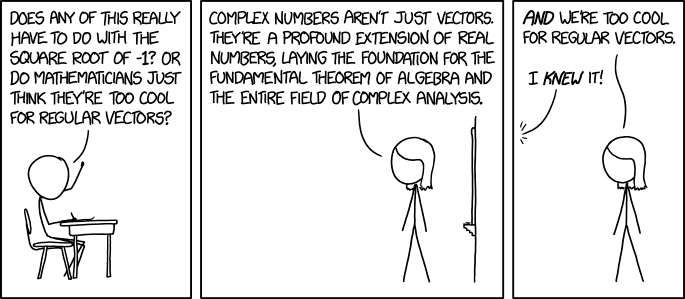
\includegraphics[scale=0.5]{xkcd_complex_numbers.png}
    \caption{Comic from https://xkcd.wtf/2028/}
\end{figure}

\begin{proposition}[Trigonometric Identities]
    Let $A$ and $B$ denote angles.
    \begin{enumerate}
        \item \textit{Pythagorean Identity}: $\sin^2A+\cos^2A=1$
        \begin{enumerate}
            \item $\tan^2A+1=\sec^2A$,
            \item $\cot^2A+1=\csc^2A$.
        \end{enumerate}
        \item Addition Formulae
        \begin{enumerate}
            \item $\sin(A\pm B)=\sin A\cos B\pm \cos A\sin B$,
            \item $\cos(A\pm B)=\cos A\cos B\mp \sin A\sin B$,
            \item $\tan(A\pm B)=\frac{\tan A\pm\tan B}{1\mp \tan A\tan B}.$
        \end{enumerate}
        \item Double Angle Formulae
        \begin{enumerate}
            \item $\sin 2A=2\sin A\cos A$,
            \item $\cos 2A=\cos^2A-\sin^2A=2\cos^2A-1=1-2\sin^2A,$
            \item $\tan 2A=\frac{2\tan A}{1-\tan^2 A}.$
        \end{enumerate}  
        \item Sum-to-Product Formulae
        \begin{enumerate}
            \item $\sin A+\sin B=2\sin\left(\frac{A+B}{2}\right)\cos\left(\frac{A-B}{2}\right),$
            \item $\sin A-\sin B=2\cos\left(\frac{A+B}{2}\right)\sin\left(\frac{A-B}{2}\right),$
            \item $\cos A+\cos B=2\cos\left(\frac{A+B}{2}\right)\cos\left(\frac{A-B}{2}\right),$
            \item $\cos A-\cos B=-2\sin\left(\frac{A+B}{2}\right)\sin\left(\frac{A-B}{2}\right).$
        \end{enumerate}
    \end{enumerate}
\end{proposition}
\begin{proposition}[Trigonometric R Method (or R-formula)]
    Let $a,b,\theta$ be reals. The R-formula expresses the \textit{weighted sum} $a\sin\theta+b\cos\theta$ as a single $\sin$ or $\cos$ term.

    Letting $R=\sqrt{a^2+b^2}$ and $\tan\alpha=\frac{b}{a}$,
    \begin{enumerate}
        \item \textit{Sine form:} $a\sin\theta\pm b\cos\theta=R\sin(\theta\pm\alpha).$
        \item \textit{Cosine form:} $a\cos\theta\pm b\sin\theta=R\cos(\theta\mp\alpha).$
    \end{enumerate}
\end{proposition}
\subsection{Applying Identities \ez}
For fundamentals, it is important that we are able to simplify complicated expressions into simpler forms.
\begin{example}
    Simplify $\cos{49^{\dg}}+\cos{71^{\dg}}$ as a single trigonometric term.
\end{example}
\begin{proof}
    Observe the symmetry about $60$: $49=60-11$ and $71=60+11$, so
    \begin{align*}
        \cos{49^{\dg}}+\cos{71^{\dg}}&=\cos{(60-11)^{\dg}}+\cos{(60+11)^{\dg}} \\
        &=2\cos{60^{\dg}}\cos{11^{\dg}} \\
        &=\boxed{\cos{11^{\dg}}}.
    \end{align*}
\end{proof}

\begin{proposition}[Toolkit]
    There usually isn't much to do with trigonometry. Most useful properties relate the sum or difference of angles, and so the usual techniques go by:
    \begin{enumerate}
        \item squaring and adding the given relations,
        \item squaring and subtracting the given relations,
        \item simply adding or subtracting the given relations,
        \item multiplying the given relations, 
        \item using sum-to-product formulae, or
        \item expressing the required expression in terms of the given angles.
    \end{enumerate}
\end{proposition}

\begin{example}[2020 SMO(S) P9]
If $8\cos{x}-8\sin{x}=3$, find the value of $\tan{x}+\frac{1}{\tan{x}}$.
\end{example}
\begin{proof}
    Firstly, $(8\cos{x}-8\sin{x})^2=64-64\sin{2x}=9 \implies \sin{2x}=\frac{55}{64}$.
    
    Moreover, $$\tan{x}+\frac{1}{\tan{x}}=\frac{\sin{x}}{\cos{x}}+\frac{\cos{x}}{\sin{x}}=\frac{2}{\sin{2x}}=\boxed{\frac{128}{55}}.$$
\end{proof}

\begin{example}[2021 SMO(O) P1]
    It is given that $\frac{\pi}{2}<\beta<\alpha<\frac{3\pi}{4}$, $\cos{(\alpha-\beta)}=\frac{12}{13}$ and $\sin{(\alpha+\beta)}=-\frac{3}{5}$. Find $\floor{|2021\sin{2\alpha}|}$.
\end{example}
\begin{proof}
    From the angle conditions, we have $0<\alpha-\beta<\frac{\pi}{4}$ and $\pi<\alpha+\beta<\frac{3\pi}{2}$. We now pull a big sneaky! Note that 
    \begin{align*}
        \sin{2\alpha}&=\sin{((\alpha-\beta)+(\alpha+\beta))} \\
        &=\sin{(\alpha-\beta)}\cos{(\alpha+\beta)}+\cos{(\alpha-\beta)}\sin{(\alpha+\beta)} \\
        &=\frac{5}{13}\cdot\left(-\frac{4}{5}\right)+\frac{12}{13}\cdot\left(-\frac{3}{5}\right) \\
        &=-\frac{4}{13}-\frac{36}{65} \\
        &=-\frac{56}{65}.
    \end{align*}
    Thus, $$\floor{|2021\sin{2\alpha}|}=\floor{\frac{2021\cdot56}{65}}=\floor{\frac{113176}{65}}=\boxed{1741}.$$
\end{proof}


\begin{example}[2021 SMO(O) P12]
    Given that $\sin{\alpha}+\sin{\beta}=\frac{1}{10}$ and $\cos{\alpha}+\cos{\beta}=\frac{1}{9}$. Find the value of $\floor{\tan^2(\alpha+\beta)}$.
\end{example}
\begin{proof}
    By the sum-to-product formulae,
    $$\frac{\sin{\alpha}+\sin{\beta}}{\cos{\alpha}+\cos{\beta}}=\tan{\left(\frac{A+B}{2}\right)}=\frac{9}{10}.$$

    Thus,
    \begin{align*}
        \floor{\tan^2{(\alpha+\beta)}}&=\floor{\left(\frac{2\tan{\left(\frac{A+B}{2}\right)}}{1-\tan^2{\left(\frac{A+B}{2}\right)}}\right)^2}\\
        &=\floor{\left(\frac{2\cdot\frac{9}{10}}{1-\frac{81}{100}}\right)^2}\\
        &=\floor{\left(\frac{180}{19}\right)^2}=\floor{\frac{32400}{361}}
        &=\boxed{89}.
    \end{align*}
\end{proof}

\begin{example}[2021 SMO(O) P15]
    Assume that $ABC$ is an acute triangle with $\sin(A+B)=\frac{3}{5}$ and $\sin(A-B)=\frac{1}{5}$. If $AB=2022(\sqrt{6}-{2})$, determine $\floor{h}$, where $h$ is the height of the triangle from $C$ to $AB$.
\end{example}
\begin{proof}
    We have that 
    \begin{align*}
        AB&=h\left(\cot{A}+\cot{B}\right) \\
        &=h\left(\frac{\cos{A}}{\sin{A}}+\frac{\cos{B}}{\sin{B}}\right) \\
        &=h\left(\frac{\sin{A}\cos{B}+\cos{A}\sin{B}}{\sin{A}\sin{B}}\right) \\
        &=h\left(\frac{2\sin(A+B)}{\cos{(A-B)}-\cos{(A+B)}}\right) \\
        &=h\left(\frac{\frac{6}{5}}{\frac{2\sqrt{6}}{5}-\frac{4}{5}}\right) \\
        &=h\left(\frac{3}{\sqrt{6}-2}\right) \\
    \end{align*}
    Thus, 
    $$h=\frac{2022(\sqrt{6}-2)}{\frac{3}{\sqrt{6}-2}}=674(\sqrt{6}-2)^2=1348(5-2\sqrt{6}).$$

    Finally, $2.4<\sqrt{6}<2.45 \implies 5-2\cdot 2.45=0.1<5-2\sqrt{6}<5-2\cdot2.4=0.2$
\end{proof}

\begin{example}[2021 SMO(S) P7]
    If $\cos{A}-\cos{B}=\frac{1}{2}$ and $\sin{A}-\sin{B}=-\frac{1}{4}$, find the value of $100\sin{(A+B)}.$
\end{example}
\begin{proof}
    With some foresight, we notice that squaring and then summing or subtracting the relations wouldn't be too useful at this point.

    We turn to the sum-to-product formulae:
    \begin{equation}\label{trig-p7-1}
        \cos{A}-\cos{B}=\frac{1}{2} \implies \sin{\frac{A+B}{2}}\sin{\frac{A-B}{2}}=-\frac{1}{4},
    \end{equation}
    and 
    \begin{equation}\label{trig-p7-2}
        \sin{A}-\sin{B}=-\frac{1}{4} \implies \cos{\frac{A+B}{2}}\sin{\frac{A-B}{2}}=-\frac{1}{8}.
    \end{equation}

    Now, squaring seems like a good idea:
    $$\eqref{trig-p7-1}^2+\eqref{trig-p7-2}^2=\sin^2{\frac{A-B}{2}=\frac{5}{64}}.$$
    Moreover, 
    $$\eqref{trig-p7-1}\cdot\eqref{trig-p7-2}=\frac{1}{2}\sin{A+B}\sin{\frac{A-B}{2}}=\frac{1}{32}.$$
    Thus, $100\sin(A+B)=100\cdot\frac{4}{5}=80.$
\end{proof}

\begin{example}[2018 SMO(S) P17]
    Let 
    $$L=\sum_{k=7}^{16}\left(1+\tan(15k^{\dg}+15^{\dg})\tan15k^{\dg}\right).$$
    Find $\floor{L}$.
\end{example}
\begin{proof}
    We see that the expression is dominated by tangents, and that the summand resembles the denominator of the tangent addition formula!

    For simplicity, let $A=15k^{\dg}+15^{\dg}$ and $B=15k^{\dg}$, then $L=\sum_{k=7}^{16}\left(1+\tan{A}\tan{B}\right).$

    To simplify this sum, consider 
    \begin{align*}
        L\cdot\tan(A-B)&=L\cdot\tan 15^{\dg}\\
        &=\sum_{k=7}^{16}\tan{(A-B)}\left(1+\tan{A}\tan{B}\right) \\
        &=\sum_{k=7}^{16} \left(\tan{A}-\tan{B}\right)=\sum_{k=7}^{16} \left(\tan{\left(15k^{\dg}+15^{\dg}\right)}-\tan{15k^{\dg}}\right)\\
        &=\left(\tan{120^{\dg}}-\tan{105^{\dg}}\right)+\left(\tan{135^{\dg}}-\tan{120^{\dg}}\right)+\cdots+\left(\tan{255^{\dg}}-\tan{240^{\dg}}\right) \\
        &=\tan{255^{\dg}}-\tan{105^{\dg}} \\
        &=2\tan{75^{\dg}}
    \end{align*}
    To this end, we first compute $\tan{15^{\dg}}$:
    $$\tan{30^{\dg}}=\frac{\sqrt{3}}{3}=\frac{2\tan{15^{\dg}}}{1-\tan^2{15^{\dg}}} \implies \tan{15^{\dg}}=2-\sqrt{3}.$$
    Then, 
    \begin{align*}
        L&=\frac{2\tan{75^{\dg}}}{\tan{15^{\dg}}}=\frac{2\tan{(30+45)^{\dg}}}{2-\sqrt{3}} \\
        &=\frac{4+2\sqrt{3}}{2-\sqrt{3}}\cdot\frac{2+\sqrt{3}}{2+\sqrt{3}}\\
        &=14+8\sqrt{3}.
    \end{align*}
    Finally, since $1.7<\sqrt{3}<1.75$,
    $$14+8\cdot1.7=27.6 < L=14+8\sqrt{3} < 14+8\cdot1.75=28,$$
    thus $\floor{L}=\boxed{27}$.
\end{proof}

\begin{example}[2021 SMO(S) P15]
    Find the minimum value of $$\frac{8}{\sin{2\theta}}+12\tan{\theta},$$
    where $0<\theta<\frac{\pi}{2}.$
\end{example}
\begin{proof}
    \begin{align*}
        \frac{8}{\sin{2\theta}}+12\tan{\theta}&=\frac{4+12\sin^2{\theta}}{\sin{\theta}\cos{\theta}} \\
        &=\frac{16\sin^2{\theta}+4\cos^2{\theta}}{\sin{\theta}\cos{\theta}} \\
        &\geq \frac{2\sqrt{64\sin^2{\theta}\cos^2{\theta}}}{\sin{\theta}\cos{\theta}} \quad\text{by AM-GM}\\
        &=\boxed{16}.
    \end{align*}
    Equality occurs when $4\cos^2{\theta}=16\sin^2{\theta} \implies \tan{\theta}=\frac{1}{2}$, for which $\theta$ lies in the given domain.
\end{proof}

\subsection{Sums and Products \med}
As a disclaimer, some parts of this section may tie into complex numbers, so you may wish to omit these parts until you have had some form of treatment on the connection between complex numbers and trigonometry.

That said, most of this section should be self-contained, and we do our best to not tie into complex numbers, although sometimes they may be used as motivation. This is just a testament to the interconnectedness between these two beautiful ideas!

\begin{example}[2014 SMO(S) P33]
    Find the value of $$2\tan{1^{\dg}}(\sin{2^{\dg}}+\sin{4^{\dg}}+\cdots+\sin{178^{\dg}}).$$    
\end{example}
With some foresight, we first note the useful identity that \begin{equation}\label{trig-p33-1}
    \cos{A-1}+\cos{A+1}=2\cos{A}\cos{1}
\end{equation}
\begin{proof}
    Let $S=\sin{2^{\dg}}+\sin{4^{\dg}}+\cdots+\sin{178^{\dg}}$,
    then 
    \begin{align*}
        S&=2(\sin{2^{\dg}}+\sin{4^{\dg}}+\cdots+\sin{178^{\dg}}+\sin{180^{\dg}}) \\
        &=2(\sin{2^{\dg}}+\sin{4^{\dg}}+\cdots+\sin{88^{\dg}})+1\\
        &=2(\cos{2^{\dg}}+\cdots)+(\cos{0^{\dg}}+\cos{90^{\dg}})\\
        &=(\cos{0^{\dg}}+\cos{2^{\dg}})+(\cos{2^{\dg}}+\cos{4^{\dg}})+\cdots+(\cos{88^{\dg}}+\cos{90^{\dg}})\\
        &=2\cos{1^{\dg}}(\cos{1^{\dg}}+\cos{3^{\dg}}+\cdots+\cos{89^{\dg}}) \quad\text{using \eqref{trig-p33-1}}\\
    \end{align*}
    Now, we use a trick to simplify the terms:
    \begin{align*}
        S&=\cot{1^{\dg}}(2\sin{1^{\dg}}\cos{1^{\dg}}+2\sin{3^{\dg}\cos{1}+\cdots+2\sin{89^{\dg}}}\cos{1}) \\
        &=\cot{1^{\dg}}((\sin{2^{\dg}}-\sin{0^{\dg}})+(\sin{4^{\dg}-\sin{2^{\dg}}})+\cdots+(\sin{90^{\dg}}-\sin{88^{\dg}}))\\
        &=\cot{1^{\dg}}(\sin{90^{\dg}}-\sin{0^{\dg}})=\cot{1^{\dg}}.
    \end{align*}
    Hence, the required value is $\boxed{2}$.
\end{proof}
\begin{example}[2013 AIME I/14]
    For $\pi\leq\theta\leq2\pi,$ let
    $$P=\frac{1}{2}\cos{\theta}-\frac{1}{4}\sin{2\theta}-\frac{1}{8}\cos{3\theta}+\frac{1}{16}\sin{4\theta}+\frac{1}{32}\cos{5\theta}-\frac{1}{64}\sin{6\theta}-\frac{1}{128}\cos{7\theta}+\cdots$$
    and
    $$Q=1-\frac{1}{2}\sin{\theta}-\frac{1}{4}\cos{2\theta}+\frac{1}{8}\sin{3\theta}+\frac{1}{16}\cos{4\theta}-\frac{1}{32}\sin{5\theta}-\frac{1}{64}\cos{6\theta}+\frac{1}{128}\sin{7\theta}+\cdots$$
    so that $\frac{P}{Q}=\frac{2\sqrt{2}}{7}.$ Find the value of $\sin{\theta}$.
\end{example}
Surely $P$ and $Q$ are connected by some obscure relation - this is almost by design! For the confused reader (I sure was!) who can't spot the pattern just yet, the terms in $P$ and $Q$ have signs that oscillate in the pattern of $(+,-,-,+)$, while the trigonometric terms oscillate between $\sin$ and $\cos$.

The terms in $P$ and $Q$ are quite unruly, so let us attempt to line them up. A naive attempt would be to first "unify" the $\cos{\theta}$ term from $P$ and the $\sin{\theta}$ term from $Q$ by considering $P\cdot\sin{\theta}$ and $Q\cdot\cos{\theta}$.

Now, for each term in $P$ and $Q$ with the same coefficient, note that we have the identities
$$\begin{cases}
    \sin{n\theta}\cos{\theta}+\cos{n\theta}\sin{\theta}=\sin{(n+1)\theta} \\
    \cos{n\theta}\sin{\theta}-\sin{n\theta}\cos{\theta}=\cos{(n+1)\theta}.
\end{cases}$$
Somehow, we now have the miraculous identity:
$$P\cdot\sin{\theta}-Q\cdot\cos{\theta}=-2P.$$

Dividing across by $Q$ yields $$\frac{P}{Q}=\frac{\cos{\theta}}{\sin{\theta}+2}=\frac{2\sqrt{2}}{7},$$
and squaring and simplifying produces the quadratic
$$57\sin^2{\theta}+32\sin{\theta}-17=0 \implies (19\sin{\theta}+17)(3\sin{\theta}-1)=0.$$
Since $\pi\leq\theta\leq2\pi$, $\sin{\theta}<0$ so $\sin{\theta}=\boxed{-\frac{17}{19}}$ only.
\subsection{Parametrising \med}
Consider the unit circle $x^2+y^2=1$. Then, we may describe the set of points along the circumference of the circle as
$$(x,y)=(\cos\theta, \sin\theta), \quad -\pi\leq\theta\leq\pi.$$
We say that this is a \textit{parametrisation} of the set of points on the circle.

And certainly, the circle $x^2+y^2=r^2$ with radius $r$ is simply a scaled unit circle, so it's points can be described as
$$(x,y)=(r\cos\theta, r\sin\theta), \quad -\pi\leq\theta\leq\pi.$$

This idea is extremely useful to re-parametrise conditions and to maximise or minimise the so-called objective functions.
\begin{example}[2018 SMO(S) P11]
    Let $x$ and $y$ be real numbers. Find the maximum value of $2x^2-3xy-2y^2$ subject to the condition that
    $$25x^2-20xy+40y^2=36.$$
\end{example}
The "cross-term" $20xy$ suggests that we should complete the square. 


\begin{proof}
    Write $$25x^2-20xy+40y^2=(25x^2-20xy+4y^2)+36y^2=(5x-2y)^2+36y^2=36.$$
    
    Now, let $36a^2=(5x-2y)^2$, then $36a^2+36y^2=36 \implies a^2+y^2=1$, and so we may parametrise 
    $$(a,y)=(\cos\theta,\sin\theta),\quad -\pi\leq\theta\leq\pi \implies (x,y)=\left(\frac{6\cos\theta+2\sin\theta}{5}, \sin\theta\right).$$
    
    Thus, \begin{align*}
        2x^2-3xy-2y^2&=\frac{2(6\cos\theta+2\sin\theta)^2-15(6\cos\theta+2\sin\theta)\sin\theta-50\sin^2\theta}{25} \\
        &=\frac{2(36\cos^2\theta+12\sin 2\theta+4\sin^2\theta)-(45\sin2\theta+30\sin^2\theta)-50\sin^2\theta}{25} \\
        &=\frac{72\cos^2\theta-72\sin^2\theta-21\sin2\theta}{25} \\
        &=\frac{72\cos2\theta-21\sin2\theta}{25} \\
        &=\frac{\sqrt{72^2+21^2}\cos(2\theta+\alpha)}{25}, \quad \text{where }\tan\alpha=\frac{21}{72} \\
        &\geq\frac{\sqrt{72^2+21^2}}{25}=\boxed{3}.
    \end{align*}
    
    The minimum occurs when $2\theta=-\tan^{-1}\frac{21}{72}$, which lies in the domain of $\theta$.
\end{proof}
\end{document}